\documentclass[11pt,a4paper]{article}

\usepackage[utf8]{inputenc}
\usepackage[T1]{fontenc}
\usepackage{amsmath,amssymb,amsthm}
\usepackage{booktabs}
\usepackage{array}
\usepackage{tikz}
\usepackage{pgfplots}
\pgfplotsset{compat=1.16}
\usepackage[margin=2.5cm]{geometry}
\usepackage[colorlinks=true,linkcolor=blue!50!black,citecolor=blue!50!black,urlcolor=blue!50!black]{hyperref}

\newtheorem{theorem}{Theorem}
\theoremstyle{definition}
\newtheorem{definition}{Definition}
\theoremstyle{remark}
\newtheorem*{remark}{Remark}

\newcommand{\hb}{\hbar}
\newcommand{\ket}[1]{|#1\rangle}
\newcommand{\bra}[1]{\langle #1|}
\newcommand{\braket}[2]{\langle #1|#2\rangle}
\newcommand{\ev}[1]{\langle #1\rangle}
\newcommand{\Z}{\mathbb{Z}}

\title{When Does Spontaneous Symmetry Breaking Need\\ Infinitely Many Degrees of Freedom?\\[4pt]
\large The double well in classical mechanics, statistical mechanics and quantum mechanics}
\author{}
\date{}

\emergencystretch=2em
\nocite{BR,Coleman,LL,Golubitsky}
\begin{document}
\maketitle

\begin{abstract}
\noindent
Spontaneous symmetry breaking (SSB) is usually introduced with a potential that has a symmetric but unstable
critical point and a pair of stable, mutually reflected minima. Whether this finite-dimensional picture
\emph{is} SSB depends on which object is required to be asymmetric. For isolated classical dynamics the object
is a single solution, and the double well is a genuine and robust example: no infinite limit is needed. For
equilibrium ensembles (classical statistical mechanics) and for quantum ground states, averaging or
superposition restores the symmetry: the Gibbs state is symmetric, the quantum ground state is unique and
symmetric, and the ``broken'' states survive only for a time exponentially long in the barrier. A sharp notion
of broken symmetry then exists only for infinitely many degrees of freedom, where the pure phases become
disjoint. We prove the quantum statement, give the Gibbs analogue, and show how both turn into true SSB for
$N$ coupled wells as $N\to\infty$.
\end{abstract}

\section{What it means for a symmetry to break}\label{sec:def}

Let $G$ be a symmetry group of the dynamics: classically a group of canonical transformations of phase space
with $H\circ g=H$, quantum mechanically a group of unitaries with $U(g)HU(g)^{-1}=H$. In both cases $G$ acts on the
algebra $\mathcal A$ of observables by automorphisms $\alpha_g$ that commute with time evolution. SSB says that
the \emph{dynamics} is symmetric but the \emph{situation the system actually finds itself in} is not. What that
situation is depends on the setting:

\begin{itemize}
\item[(A)] \textbf{Isolated classical system.} A probability measure on phase space that is invariant under the
Hamiltonian flow: a Dirac measure at an equilibrium point, the ergodic measure on an energy shell, and so on.
(A single trajectory is a special case.)
\item[(B)] \textbf{Classical system in thermal equilibrium.} The Gibbs measure $e^{-\beta H}/Z$.
\item[(C)] \textbf{Quantum system.} The ground state, or at $T>0$ a Gibbs/KMS state.
\end{itemize}

We call all of these \emph{equilibrium states}. They form a convex set. A state $\omega$ is \emph{symmetric}
if $\omega\circ\alpha_g=\omega$ for all $g$, and a \emph{phase} is an extremal equilibrium state, one that is
not a nontrivial mixture of others.

The naive definition ``the equilibrium state is not symmetric'' is not good enough. If $\omega$ is an equilibrium
state, so is $\omega\circ\alpha_g$, and the symmetrised mixture $\int dg\,\omega\circ\alpha_g$ is a symmetric
equilibrium state. So a symmetric state always exists. Moreover, in quantum mechanics a degenerate ground
multiplet contains non-symmetric pure states without any symmetry being ``broken'': every superposition of them
is again a ground state and observables connect them (the hydrogen $2p$ level is not a case of SSB). What
matters is whether the non-symmetric phases are \emph{physically disconnected}.

\begin{definition}[SSB]\label{def:ssb}
Two states are \emph{disjoint} if their GNS representations are disjoint; for classical states
(probability measures) this means they are mutually singular, and in either case no observable has a nonzero
matrix element or overlap between them. The symmetry is \emph{spontaneously broken} if there is a phase
$\omega$ with $\omega\circ\alpha_g\neq\omega$ for some $g$ and with $\omega\circ\alpha_g$ disjoint from
$\omega$.
\end{definition}

This single definition has different consequences according to the algebra $\mathcal A$:

\begin{enumerate}
\item \textbf{Classical (commutative algebra of phase-space functions).} Distinct extremal states are
mutually singular, so disjointness is \emph{automatic}. Whether SSB occurs only depends on whether the set of
equilibrium states contains several phases.
\item \textbf{Quantum, finitely many degrees of freedom.} The algebra has a unique irreducible representation
(Stone--von Neumann), so every pure state is a vector state of the same irreducible representation and two
different ones are \emph{never} disjoint. Hence no SSB at all, however degenerate the ground space is.
\item \textbf{Quantum or classical-statistical, infinitely many degrees of freedom.} The quasi-local
algebra has uncountably many inequivalent representations, and distinct pure phases can be disjoint.
\end{enumerate}

In an infinite system the order parameter, such as $m=\lim_N N^{-1}\sum_ix_i$, is not a local observable but
commutes with all local ones (a tail variable classically, a central element quantum mechanically). It takes the
sharp value $\pm m_0$ in the pure phases, which is what a superselection variable is. See~\cite{Strocchi,Haag}
for the algebraic treatment.

So the question is, for each of (A), (B), (C): does the \emph{finite} system already have several phases?
In (A) yes, in (B) and (C) no. That is the content of the article.

\section{Classical mechanics: SSB with finitely many degrees of freedom}\label{sec:classical}

\subsection{The system}

Take the one-dimensional system
\begin{equation}
H=\frac{p^2}{2m}+V(x),\qquad V(x)=\lambda\,(x^2-a^2)^2,
\label{eq:H}
\end{equation}
with the parity symmetry $G=\Z_2$ generated by $P:(x,p)\to(-x,-p)$, $H\circ P=H$.

The equilibria are $x=0$ with $V''(0)=-4\lambda a^2<0$ (a local maximum of height $V_0=\lambda a^4$, a saddle
point of the phase-space flow with exponential growth rate $\kappa=\sqrt{4\lambda a^2/m}=\omega/\sqrt2$), and
$x=\pm a$ with $V''(\pm a)=8\lambda a^2>0$ (two centres with small-oscillation frequency
$\omega=\sqrt{8\lambda a^2/m}$). Figure~\ref{fig:classical} shows the potential and the phase portrait.

\begin{figure}[t]
\centering
\begin{minipage}[t]{0.48\textwidth}
\centering
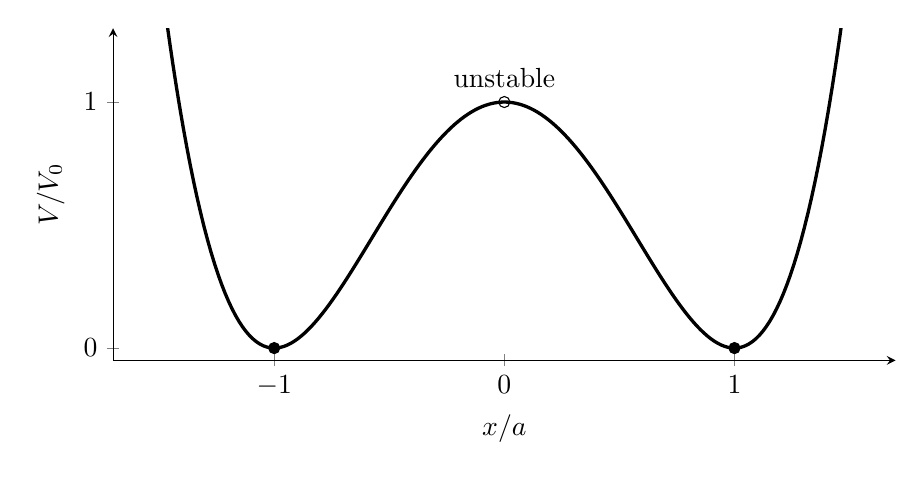
\begin{tikzpicture}
\begin{axis}[
  width=0.95\linewidth, height=5.8cm,
  axis lines=left, xlabel={$x/a$}, ylabel={$V/V_0$},
  xmin=-1.7, xmax=1.7, ymin=-0.05, ymax=1.3,
  ytick={0,1}, xtick={-1,0,1}, samples=200]
  \addplot[very thick, black, domain=-1.5:1.5] {(x^2-1)^2};
  \addplot[only marks, mark=*, mark size=2pt] coordinates {(-1,0) (1,0)};
  \addplot[only marks, mark=o, mark size=2pt] coordinates {(0,1)};
  \node[anchor=south] at (axis cs:0,1.02) {unstable};
\end{axis}
\end{tikzpicture}
\end{minipage}\hfill
\begin{minipage}[t]{0.48\textwidth}
\centering
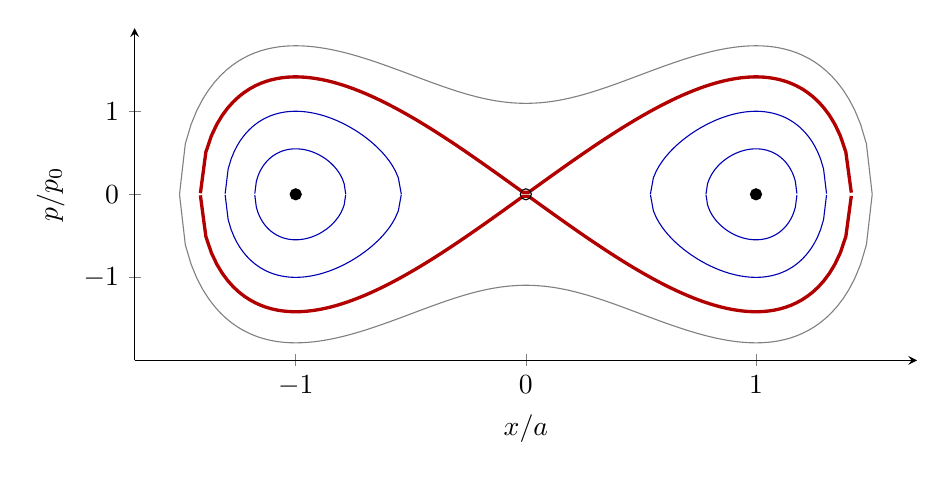
\begin{tikzpicture}
\begin{axis}[
  width=0.95\linewidth, height=5.8cm,
  axis lines=left, xlabel={$x/a$}, ylabel={$p/p_0$},
  xmin=-1.7, xmax=1.7, ymin=-2, ymax=2,
  xtick={-1,0,1}, ytick={-1,0,1}]
  \foreach \E in {0.15,0.5}{
    \pgfmathsetmacro{\xa}{sqrt(1-sqrt(\E))}
    \pgfmathsetmacro{\xb}{sqrt(1+sqrt(\E))}
    \foreach \sg in {1,-1}{
      \addplot[blue!70!black, domain=\xa:\xb, samples=60]
        ({\sg*x},{sqrt(max(0,2*(\E-(x^2-1)^2)))});
      \addplot[blue!70!black, domain=\xa:\xb, samples=60]
        ({\sg*x},{-sqrt(max(0,2*(\E-(x^2-1)^2)))});
    }
  }
  \addplot[very thick, red!70!black, domain=-1.4142:1.4142, samples=120]
    ({x},{sqrt(max(0,2*(1-(x^2-1)^2)))});
  \addplot[very thick, red!70!black, domain=-1.4142:1.4142, samples=120]
    ({x},{-sqrt(max(0,2*(1-(x^2-1)^2)))});
  \addplot[gray, domain=-1.505:1.505, samples=120]
    ({x},{sqrt(max(0,2*(1.6-(x^2-1)^2)))});
  \addplot[gray, domain=-1.505:1.505, samples=120]
    ({x},{-sqrt(max(0,2*(1.6-(x^2-1)^2)))});
  \addplot[only marks, mark=*, mark size=2pt] coordinates {(-1,0) (1,0)};
  \addplot[only marks, mark=o, mark size=2pt] coordinates {(0,0)};
\end{axis}
\end{tikzpicture}
\end{minipage}
\caption{Left: the double well~\eqref{eq:H}. Right: its phase portrait in units $m=\lambda=a=1$
($p_0=\sqrt{m\lambda}\,a^2$). For $E<V_0$ the energy shell has two disconnected components (blue), swapped by
$P$; at $E=V_0$ it is the figure-eight separatrix through the saddle (red); for $E>V_0$ a single component
encircles both wells (grey).}
\label{fig:classical}
\end{figure}

\subsection{Solutions are asymmetric}

For $E<V_0$ the energy shell $\{H=E\}$ has two connected components $\Sigma_E^\pm$ (the sign of $x$), each a
single periodic orbit, and $P$ maps $\Sigma^+_E$ onto $\Sigma^-_E$. A solution lives in one component for all
time: it never changes sign of $x$, because $x=0$ is not reachable at that energy. Hence \emph{no solution with
$E<V_0$ is invariant under $P$}: the image of a solution is a different solution, in the other well.
The only symmetric equilibrium is $x\equiv0$, which has $E=V_0$ and is unstable with rate $\kappa$. Symmetric
solutions (orbits mapped to themselves) exist only at $E\ge V_0$.

In the language of Section~\ref{sec:def}: the phases are the Dirac measures at $(\pm a,0)$ and the ergodic
measures on the shells $\Sigma^\pm_E$, $E<V_0$. They are not $P$-invariant, they are mutually singular, and the
$P$-symmetric measure $\tfrac12(\delta_{(a,0)}+\delta_{(-a,0)})$ is invariant but not extremal, i.e.\ it is a
mixture which describes our ignorance, not a state the system can be in. So Definition~\ref{def:ssb} is met by a system with a single coordinate.

\subsection{Robustness: hysteresis}

The asymmetric solutions are structurally stable. Perturb the Hamiltonian by a symmetry-breaking
field, $H_h=H-hx$. Then $V_h'(x)=4\lambda x(x^2-a^2)-h$ has three real roots, two stable and one unstable, for all
\begin{equation}
|h|<h_c=\frac{8\lambda a^3}{3\sqrt3},
\label{eq:hc}
\end{equation}
so a system in the well $x\approx a$ stays there when $h$ is swept through $0$ down to $-h_c$. The
order parameter is \emph{two-valued} at $h=0$: $\lim_{h\to0^\pm}x_*(h)=\pm a$ for the stable equilibrium
reached from either side, which is hysteresis. This is exactly the behaviour which the ground state of a
finite quantum system does \emph{not} have (Section~\ref{sec:quantum}), and which a finite thermal ensemble does not
have either (Section~\ref{sec:stat}).

\begin{remark}
Unfolding the potential as $V_\mu=-\mu x^2/2+\lambda x^4$ and letting $\mu$ pass through $0$ gives the
pitchfork bifurcation, the classical normal form of symmetry breaking~\cite{Golubitsky}: the symmetric
equilibrium loses stability and two asymmetric ones appear. No limit $N\to\infty$ is involved. The textbook
statement ``the symmetric state is unstable, so the system picks a side'' is correct here, because a classical
state is a point in phase space, there is no superposition principle, and nothing averages the two wells.
\end{remark}

\section{Classical statistical mechanics: the Gibbs state is symmetric}\label{sec:stat}

\subsection{One well}

Put the system of Section~\ref{sec:classical} in contact with a heat bath at inverse temperature $\beta$ (for
instance Langevin dynamics with friction). The equilibrium state is the Gibbs measure
$\mu_\beta\propto e^{-\beta H}\,dx\,dp$. It is $P$-symmetric, so $\ev{x}=0$ at every temperature, and for
Langevin dynamics with a confining potential it is the \emph{unique} invariant probability measure. Hence it
is ergodic, i.e.\ extremal: there is exactly one phase, and it is symmetric. By Definition~\ref{def:ssb} the
finite thermal double well does not break the symmetry.

The decomposition one is tempted to make, $\mu_\beta\simeq\tfrac12(\mu_++\mu_-)$ with $\mu_\pm$ the restrictions
to $\pm x>0$ (accurate when $\beta V_0\gg1$), is not a decomposition into phases because $\mu_\pm$ are not
invariant. The trajectories cross the barrier at the transition-state or Kramers rate
\begin{equation}
r\;\simeq\;\kappa_{\rm K}\,\frac{\omega}{2\pi}\,e^{-\beta V_0},\qquad 0<\kappa_{\rm K}\le1,
\label{eq:kramers}
\end{equation}
where $\kappa_{\rm K}$ is a friction-dependent transmission factor~\cite{Kramers,Hanggi}, and the order parameter
correlation decays as $\ev{x(t)x(0)}\simeq\ev{x^2}e^{-2rt}$. Time averages over $t\gg1/r$ give $\ev{x}=0$ (ergodicity). The
asymmetric pseudo-phases are metastable for times $\ll 1/r$, nothing more.

\paragraph{Why this differs from Section~\ref{sec:classical}.} An isolated system with $E<V_0$ \emph{never}
crosses; the crossing in~\eqref{eq:kramers} comes from energy exchange with the bath, which makes $E>V_0$
possible with Boltzmann weight $e^{-\beta V_0}$. Isolation (fixed energy below the barrier) gives SSB;
equilibration with a bath removes it, at finite size.

\subsection{\texorpdfstring{$N$}{N} coupled wells and the limit \texorpdfstring{$N\to\infty$}{N to infinity}}

Take $N$ wells with mean-field (all-to-all) ferromagnetic coupling,
\begin{equation}
H_N=\sum_{i=1}^N\Bigl[\frac{p_i^2}{2m}+V(x_i)\Bigr]-\frac{K}{2N}\Bigl(\sum_{i=1}^Nx_i\Bigr)^2,
\end{equation}
and let $m=N^{-1}\sum_ix_i$. For low enough temperature or strong enough $K$ the free energy per site
$f(m)$ has two minima at $\pm m_0$ separated by a barrier, and the probability of $m$ is $\propto e^{-\beta N[f(m)-f(m_0)]}$.
At every finite $N$ the Gibbs measure is again unique and symmetric. But the barrier is now \emph{extensive}, so the
flip rate is
\begin{equation}
r_N\;\sim\;e^{-\beta N\,[f(0)-f(m_0)]}\;\xrightarrow{N\to\infty}\;0 .
\end{equation}
Three consequences follow, each a classical shadow of what happens for quantum ground states.

\begin{itemize}
\item \textbf{Order of limits.} $\lim_{h\to0^\pm}\lim_{N\to\infty}\ev{m}_{N,h}=\pm m_0$, while
$\lim_{N\to\infty}\lim_{h\to0}\ev{m}_{N,h}=0$; likewise, the time and size limits do not commute.
\item \textbf{Disjoint phases.} By the law of large numbers, $m=\pm m_0$ almost surely in the limiting
measures $\mu_\pm$, so $\mu_+\perp\mu_-$: they are mutually singular, concentrated on disjoint sets of
configurations, and both are ergodic. Now there \emph{are} several phases, Definition~\ref{def:ssb} is met, and the
symmetric Gibbs measure converges to the non-extremal mixture $\tfrac12(\mu_++\mu_-)$ for all local observables.
\item \textbf{Clustering.} In that mixture $\ev{x_i}=0$ but $\ev{x_ix_j}-\ev{x_i}\ev{x_j}=m_0^2\ne0$ for all $i\neq j$:
the symmetric state violates cluster decomposition, and the physical states are $\mu_\pm$.
\end{itemize}

\begin{remark}
For short-range couplings on a $d$-dimensional lattice and a discrete symmetry the barrier is the cost of a
domain wall, growing like $L^{d-1}$. Thermal SSB then exists for $d\ge2$ (Peierls) but not for $d=1$, where
domain walls cost only a finite free energy, so the correlation length stays finite. The mean-field
model above is the cleanest example of the mechanism, not the only one.
\end{remark}

\section{Quantum mechanics: the finite system has a unique symmetric ground state}\label{sec:quantum}

\subsection{The theorem}

Now quantise~\eqref{eq:H}, with $P:x\to-x$ acting on wave functions.

\begin{theorem}\label{thm:nodeless}
Let $V$ be real, continuous, bounded below and confining. Then the ground state of
$H=p^2/2m+V(x)$ is nondegenerate and can be chosen strictly positive. In particular, if
$V(x)=V(-x)$, the ground state is parity-even and $\ev{x}_0=0$ exactly, for every $\hb,\lambda,a$.
\end{theorem}

\begin{proof}
For real or complex $\psi$ one has $\bigl|\,|\psi|'\,\bigr|\le|\psi'|$ almost everywhere, hence
$\braket{|\psi|}{H|\psi|}\le\braket{\psi}{H\psi}$ with the same norm. So if $\psi$ minimises the energy, so does
$|\psi|$, which is therefore an eigenfunction (and, by the Schr\"odinger equation, $C^2$). Suppose
$|\psi|(x_0)=0$. Then $|\psi|\ge0$ has a minimum at $x_0$, so $|\psi|'(x_0)=0$, and the uniqueness theorem for
the second-order ODE forces $|\psi|\equiv0$, a contradiction. So $|\psi|>0$ everywhere.

Since $H$ is real, the real and imaginary parts of a ground state are ground states, so one may restrict to real
ground states $\varphi$. Each has $|\varphi|>0$, hence $\varphi$ has a constant sign. Two functions of constant
sign cannot be orthogonal, so the ground space is one-dimensional.

Finally $P\psi_0$ is also a ground state, hence $P\psi_0=c\,\psi_0$ with $c=\pm1$; positivity gives $c=+1$.
\end{proof}

The same argument (Perron--Frobenius for the positivity-preserving semigroup $e^{-tH/\hb}$) applies to any
number $N$ of bosonic degrees of freedom with a scalar potential~\cite{ReedSimon4}. So in no such system with
a finite number of degrees of freedom does the ground state break a symmetry that maps positive functions to
positive functions, and $\ev{x}_0=0$ always. By Definition~\ref{def:ssb}, together with the uniqueness of the
irreducible representation, there are not even two candidate phases.

\subsection{What the ``broken'' states are}

\begin{figure}[t]
\centering
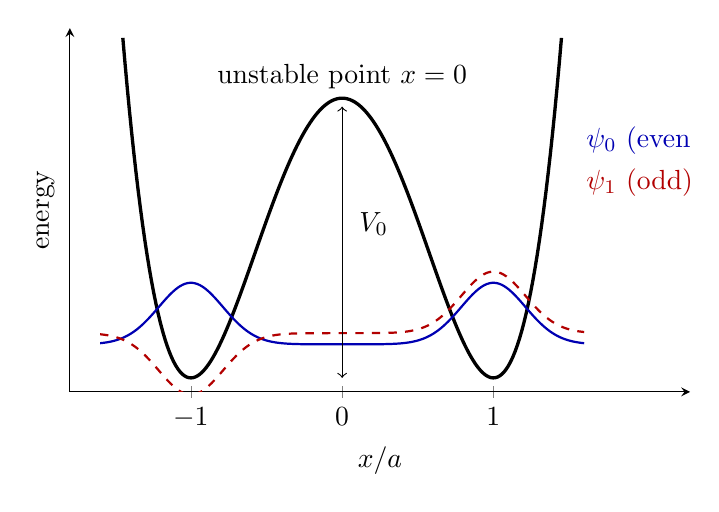
\begin{tikzpicture}
\begin{axis}[
  width=0.78\textwidth, height=6.2cm,
  axis lines=left, xlabel={$x/a$}, ylabel={energy},
  xmin=-1.8, xmax=2.3, ymin=-0.05, ymax=1.25,
  ytick=\empty, xtick={-1,0,1},
  samples=200]
  \addplot[very thick, black, domain=-1.45:1.45] {(x^2-1)^2};
  % schematic levels and wavefunctions (not to scale)
  \def\Eo{0.12}
  \def\Et{0.16}
  \addplot[thick, blue!70!black, domain=-1.6:1.6]
     {\Eo + 0.22*(exp(-((x-1)/0.3)^2)+exp(-((x+1)/0.3)^2))};
  \addplot[thick, red!70!black, dashed, domain=-1.6:1.6]
     {\Et + 0.22*(exp(-((x-1)/0.3)^2)-exp(-((x+1)/0.3)^2))};
  \node[blue!70!black, anchor=west] at (axis cs:1.55,0.85) {$\psi_0$ (even)};
  \node[red!70!black, anchor=west]  at (axis cs:1.55,0.70) {$\psi_1$ (odd)};
  \node[anchor=south] at (axis cs:0,1.0) {unstable point $x=0$};
  \draw[<->] (axis cs:0,0.0) -- (axis cs:0,0.97);
  \node[anchor=west] at (axis cs:0.05,0.55) {$V_0$};
\end{axis}
\end{tikzpicture}
\caption{The double well with the two lowest eigenfunctions drawn schematically at their energy levels
($\psi_0$ solid, $\psi_1$ dashed). The lowest state is even and has no node; the first excited state is odd, and
$\ket{R},\ket{L}=(\ket0\pm\ket1)/\sqrt2$ are the localised states. The splitting $\Delta=E_1-E_0$ is
exponentially small in $S_0/\hb$.}
\label{fig:well}
\end{figure}

The picture ``the particle sits in the right well'' does correspond to something: the first excited state
$\ket1$ is odd (one node), and
\begin{equation}
\ket R=\tfrac1{\sqrt2}(\ket0+\ket1),\qquad \ket L=\tfrac1{\sqrt2}(\ket0-\ket1)
\end{equation}
are concentrated in the right and left wells. These are \emph{not} stationary. With $\Delta=E_1-E_0$,
\begin{equation}
\ket{R(t)}=\tfrac1{\sqrt2}e^{-iE_0t/\hb}\bigl(\ket0+e^{-i\Delta t/\hb}\ket1\bigr),
\qquad \ev{x}_{R(t)}\simeq a\cos(\Delta t/\hb),
\end{equation}
so the particle tunnels from right to left in the time $t_{\rm tun}=\pi\hb/\Delta$. The semiclassical
(WKB/instanton) estimate of the splitting is
\begin{equation}
\Delta\;\sim\;\hb\omega\sqrt{\frac{S_0}{\hb}}\;e^{-S_0/\hb},\qquad
S_0=\int_{-a}^{a}\!\sqrt{2mV(x)}\,dx=\frac{4a^3}{3}\sqrt{2m\lambda},
\label{eq:split}
\end{equation}
with a prefactor of order one that depends on the shape of $V$. It is exponentially small in $S_0/\hb$ but
\emph{nonzero for every finite system}. It plays the role of the Kramers rate~\eqref{eq:kramers}: coherent
oscillation instead of incoherent hopping, but the same exponential smallness. Three observations show why this
is not SSB.

\paragraph{(i) The vacuum is symmetric.} The true ground state is $\ket0$, with $P\ket0=\ket0$ and
$\ev{x}_0=0$. Nothing was ``chosen''. The unstable classical point $x=0$ is irrelevant: stationary quantum
states are not subject to the classical instability argument, and $\ket0$ is not concentrated at $x=0$ anyway.
The mixture $\tfrac12(\delta_{(a,0)}+\delta_{(-a,0)})$ of Section~\ref{sec:classical} has no analogue as a ground
state: the symmetric combination $\ket0$ \emph{is} the ground state.

\paragraph{(ii) The states $\ket L,\ket R$ are connected by an observable.} The operator $x$ has matrix
element $\bra0x\ket1\simeq a\neq0$, and the unitary $e^{-ip\cdot 2a/\hb}$ translates $\ket L$ into
$\ket R$. By the Stone--von Neumann theorem (for finitely many degrees of freedom every regular
representation of the Weyl relations is a multiple of the Schr\"odinger one) there is a single irreducible
representation of the observable algebra. A pair of states that live in one irreducible representation are not
disjoint, so $\ket R$ and $\ket L$ cannot define superselection sectors: the superposition $\ket0$ is as
physical as either one. The classical Dirac measures at $(\pm a,0)$ are mutually singular automatically;
quantum vector states in one irreducible representation never are.

\paragraph{(iii) A small perturbation removes the distinction continuously.} Add a symmetry-breaking field,
$H_h=H-hx$. In the two-level approximation (valid for $|ha|\ll\hb\omega$), in the basis $\{\ket R,\ket L\}$
\begin{equation}
H_h\simeq E_0+\tfrac\Delta2-\tfrac\Delta2\,\sigma_x-ha\,\sigma_z
\quad\Longrightarrow\quad
\frac{\ev{x}_h}{a}=\frac{2ha}{\sqrt{\Delta^2+4h^2a^2}}.
\label{eq:crossover}
\end{equation}
For $|h|\ll\Delta/a$ the response is linear, $\ev{x}_h\simeq\chi h$ with a large but finite susceptibility
$\chi=2a^2/\Delta$; only for $|h|\gg\Delta/a$ does the particle sit in one well. In particular
$\lim_{h\to0}\ev{x}_h=0$, and this limit is \emph{continuous}, with no hysteresis, in contrast to the classical
result~\eqref{eq:hc}. Real SSB shows up as a \emph{discontinuity}: $\lim_{h\to0^\pm}\ev{m}_h=\pm m_0\neq0$.

\begin{figure}[t]
\centering
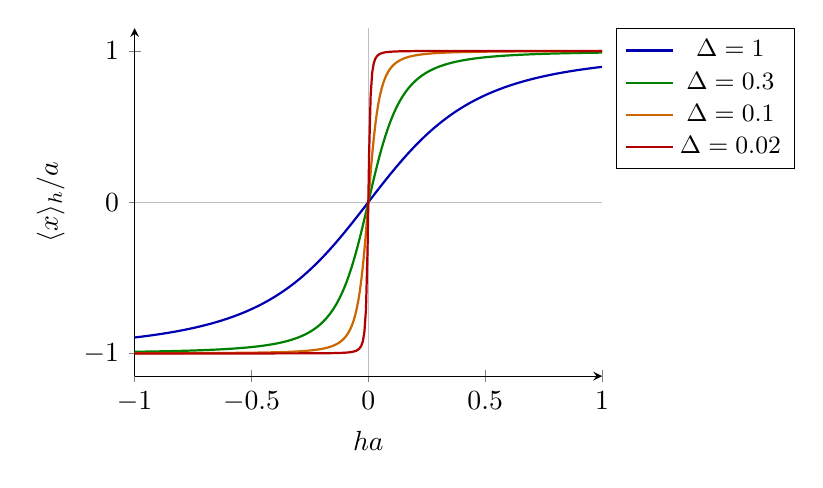
\begin{tikzpicture}
\begin{axis}[
  width=0.62\textwidth, height=6cm,
  axis lines=left, xlabel={$ha$}, ylabel={$\ev{x}_h/a$},
  xmin=-1, xmax=1, ymin=-1.15, ymax=1.15,
  xtick={-1,-0.5,0,0.5,1}, ytick={-1,0,1},
  samples=300, domain=-1:1,
  legend pos=outer north east, legend style={font=\small}]
  \draw[gray!50] (axis cs:-1,0) -- (axis cs:1,0);
  \draw[gray!50] (axis cs:0,-1.15) -- (axis cs:0,1.15);
  \addplot[thick, blue!70!black]      {2*x/sqrt(1^2+4*x^2)};
  \addplot[thick, green!50!black]     {2*x/sqrt(0.3^2+4*x^2)};
  \addplot[thick, orange!80!black]    {2*x/sqrt(0.1^2+4*x^2)};
  \addplot[thick, red!70!black]       {2*x/sqrt(0.02^2+4*x^2)};
  \legend{$\Delta=1$,$\Delta=0.3$,$\Delta=0.1$,$\Delta=0.02$}
\end{axis}
\end{tikzpicture}
\caption{Eq.~\eqref{eq:crossover} for decreasing $\Delta$ ($\Delta$ and $ha$ in units of $\hb\omega$). The
response is smooth for any $\Delta>0$ and becomes a step function only when $\Delta\to0$, which is what
happens when $N\to\infty$ in the coupled system of Section~\ref{sec:coupled}.}
\label{fig:cross}
\end{figure}

\section{Quantum wells in the limit \texorpdfstring{$N\to\infty$}{N to infinity}}\label{sec:coupled}

\subsection{A chain of coupled wells}

Take $N$ copies of the well coupled ferromagnetically,
\begin{equation}
H_N=\sum_{i=1}^N\Bigl[\frac{p_i^2}{2m}+V(x_i)\Bigr]-K\sum_{i}x_ix_{i+1},\qquad K>0,
\end{equation}
(or its spin-$\tfrac12$ caricature, the transverse-field Ising ring
$H=-J\sum_i\sigma^z_i\sigma^z_{i+1}-\Gamma\sum_i\sigma^x_i$, $\Gamma<J$), which commutes with the global
parity $P=\prod_iP_i$. The classical minima include the two homogeneous configurations $x_i\equiv\pm a'$.

For every finite $N$, Theorem~\ref{thm:nodeless} applies (for the spin ring, its Perron--Frobenius
version, since $-\Gamma\sigma^x$ has nonpositive off-diagonal elements in the $\sigma^z$ basis): the ground
state is unique, even, and has $\ev{m}=0$ where $m=N^{-1}\sum_ix_i$. We couple a field $h$ to the total
moment, $H_{N,h}=H_N-h\sum_ix_i$. To go from ``all right'' to ``all left'' by tunnelling one has to
move \emph{all $N$ coordinates} through the barrier; for the ring the dominant path is a domain wall that
travels once around it, and the action is extensive:
\begin{equation}
\Delta_N\;\sim\;e^{-sN}\qquad(s>0\ \text{the action per site}),
\label{eq:DeltaN}
\end{equation}
(for the Ising ring the splitting is $\propto(\Gamma/J)^N$). The splitting $\Delta_N\to0$ exponentially in
$N$, in parallel with the classical flip rate $r_N$ of Section~\ref{sec:stat}. In this one-dimensional quantum
chain SSB survives at $T=0$; at $T>0$ the short-range chain has none, as in the classical remark above.

\paragraph{Order of limits.} The two limits ``zero field'' and ``infinite size'' no longer commute:
\begin{equation}
\lim_{N\to\infty}\,\lim_{h\to0}\ev{m}_{N,h}=0
\qquad\text{but}\qquad
\lim_{h\to0^\pm}\,\lim_{N\to\infty}\ev{m}_{N,h}=\pm m_0\neq0 .
\end{equation}
This is Eq.~\eqref{eq:crossover} with $\Delta\to\Delta_N$, $a\to Na'$ (so the relevant combination is
$hNa'/\Delta_N$, which tends to $\infty$ for any fixed $h\neq0$). The susceptibility of the total moment,
$\chi_N\sim N^2/\Delta_N$, diverges. Likewise for time: starting from $\ket{R}$, the order parameter oscillates
with period $\sim\hb/\Delta_N$, which diverges.

\paragraph{Locality and the flip operator.} In the double well, the operator that maps $\ket L$ to $\ket R$ is
a single-particle operator, a translation. In the chain it is the global flip $\prod_iT_i$ (or
$\prod_i\sigma^x_i$), which acts on all $N$ sites. As $N\to\infty$ it ceases to be a (quasi-)local operator: no
observable that can be measured in a finite region, however large, connects the sectors. In the Ising limit
$\Gamma=0$ this is exact: the product states $\ket{\uparrow\uparrow\cdots}$ and $\ket{\downarrow\downarrow\cdots}$
satisfy
\begin{equation}
\braket{\uparrow\uparrow\cdots}{\downarrow\downarrow\cdots}=\prod_{i=1}^{\infty}\braket{\uparrow}{\downarrow}=0,
\end{equation}
and in fact any two product states that differ in infinitely many sites are orthogonal and generate
inequivalent representations (von Neumann's incomplete infinite tensor products). So Stone--von Neumann no
longer applies, the algebra of observables has uncountably many inequivalent irreducible representations,
and the disjointness required by Definition~\ref{def:ssb} becomes possible.

\paragraph{Cluster decomposition.} The symmetric ``cat state'' $\ket{\rm cat}=(\ket++\ket-)/\sqrt2$, which was
the ground state for finite $N$, has $\ev{\sigma_i}=0$ but
\begin{equation}
\ev{\sigma_i\sigma_j}-\ev{\sigma_i}\ev{\sigma_j}\;\xrightarrow{|i-j|\to\infty}\;m_0^2\neq0,
\end{equation}
so it violates clustering, the requirement that distant measurements be statistically independent in a pure
phase. All local observables have the same expectation in $\ket{\rm cat}$ as in the mixture
$\tfrac12(\omega_++\omega_-)$, because the cross terms vanish for local $A$. So in the limit it is simply a
classical mixture of two pure phases, and the physical states are $\omega_\pm$, exactly as in the classical
Gibbs case of Section~\ref{sec:stat}. The symmetric ground state of the finite system becomes a statistical
ensemble of two broken vacua, and ``the system chooses'' is meaningful because there is a superselection rule
behind the choice.

\subsection{Continuous symmetries}

The same logic holds for a continuous group, where the finite-size precursor is a \emph{tower of states}.
For a particle on the circle of minima of a Mexican hat the Hamiltonian reduces to a planar rotor,
$E_\ell=\hb^2\ell^2/2I$, with the unique rotation-invariant ground state $\ell=0$. For $N$ coupled units the
moment of inertia of the order parameter grows like $I\propto N$, so the gaps close as $1/N$. In the limit
the tower collapses onto a degenerate manifold which carries inequivalent representations and the Goldstone
modes. The ``Anderson tower of states'' is the finite-size numerical signature of SSB.

\section{Summary}

\begin{table}[ht]
\centering
\small
\renewcommand{\arraystretch}{1.25}
\newcolumntype{L}[1]{>{\raggedright\arraybackslash}p{#1}}
\begin{tabular}{@{}L{2.6cm}L{3.1cm}L{2.2cm}L{3.4cm}L{2.9cm}@{}}
\toprule
Setting & Object that must be asymmetric & SSB with finite $N$? & What restores the symmetry & Scale\\
\midrule
Classical mechanics, isolated, $E<V_0$ & trajectory / ergodic measure & \textbf{yes} & nothing (no superposition, no averaging) & --- (hysteresis, $h_c$)\\
Classical, thermal (Gibbs) & equilibrium measure & no & thermal barrier crossing & hopping rate $r\sim e^{-\beta V_0}$\\
Quantum, $T=0$ & ground state & no & superposition, uniqueness (Thm.~\ref{thm:nodeless}) & tunnelling splitting $\Delta\sim e^{-S_0/\hb}$\\
Thermal or quantum, $N\to\infty$ & extremal Gibbs or ground state & \textbf{yes}, in the limit & disjointness of phases & $r_N,\Delta_N\to0$\\
\bottomrule
\end{tabular}
\renewcommand{\arraystretch}{1}
\end{table}

\begin{table}[ht]
\centering
\small
\begin{tabular}{@{}p{4.6cm}p{5.4cm}p{5.2cm}@{}}
\toprule
 & Double well (quantum, $N=1$) & $N\to\infty$ coupled wells / spins\\
\midrule
Ground state & unique, symmetric & degenerate family of pure phases, not symmetric\\
$\ev{\text{order parameter}}$ in $\ket{0}$ & $0$ exactly & $\pm m_0$ in each phase\\
Splitting $\Delta$ & $\sim e^{-S_0/\hb}>0$ & $\sim e^{-sN}\to0$\\
Response to $h\to0$ & continuous, $\chi=2a^2/\Delta$ finite & discontinuous, $\chi=\infty$\\
Representations of observables & unique (Stone--von Neumann) & inequivalent, disjoint\\
Operator linking $L$ and $R$ & local ($x$ or $e^{-2iap/\hb}$) & global flip, nonlocal\\
Superposition of $L$ and $R$ & physical (the ground state) & mixture; violates clustering\\
\bottomrule
\end{tabular}
\end{table}

So the double well with one unstable and two stable equilibria is an example of SSB for a single classical
solution, and not an example for a classical equilibrium ensemble or for a quantum ground state. What makes the
difference is whether anything can \emph{combine} the two wells into a single state: classically nothing can, in a
thermal ensemble the heat bath does it through barrier crossings at rate $r\sim e^{-\beta V_0}$, and
quantum mechanically superposition does it through tunnelling at rate $\Delta/\hb\sim e^{-S_0/\hb}$.

The finite thermal or quantum double well displays an \emph{approximate} or \emph{effective} symmetry breaking:
if the rate is much smaller than every other scale and every time of interest is shorter than $1/r$ or
$\hb/\Delta$, the two wells behave like distinct phases. This is the situation of chiral molecules, where the
tunnelling time of a heavy chiral molecule exceeds any observation time. But that is a statement about \emph{time
scales}, not about the structure of the theory. Strict SSB of an equilibrium or ground state requires that the
rate be exactly zero, and that needs infinitely many degrees of freedom:
\begin{quote}
\emph{For thermal or quantum states, SSB $\iff$ $r_N$ (or $\Delta_N$) $\to0$ as $N\to\infty$, together with
disjoint pure phases. For isolated classical dynamics, finitely many degrees of freedom suffice.}
\end{quote}

\begin{thebibliography}{99}
\bibitem{Strocchi} F.~Strocchi, \emph{Symmetry Breaking}, Lecture Notes in Physics 643, Springer (2005).
\bibitem{Haag} R.~Haag, \emph{Local Quantum Physics}, Springer (1992).
\bibitem{BR} O.~Bratteli and D.~W.~Robinson, \emph{Operator Algebras and Quantum Statistical Mechanics}, Springer.
\bibitem{ReedSimon4} M.~Reed and B.~Simon, \emph{Methods of Modern Mathematical Physics IV: Analysis of Operators}, Academic Press (1978), Ch.~XIII.
\bibitem{Coleman} S.~Coleman, \emph{Aspects of Symmetry}, Cambridge University Press (1985).
\bibitem{LL} L.~D.~Landau and E.~M.~Lifshitz, \emph{Quantum Mechanics (Non-relativistic Theory)}, Pergamon.
\bibitem{Golubitsky} M.~Golubitsky and D.~G.~Schaeffer, \emph{Singularities and Groups in Bifurcation Theory}, Vol.~I, Springer (1985).
\bibitem{Kramers} H.~A.~Kramers, Physica \textbf{7}, 284 (1940).
\bibitem{Hanggi} P.~H\"anggi, P.~Talkner and M.~Borkovec, Rev.\ Mod.\ Phys.\ \textbf{62}, 251 (1990).
\end{thebibliography}

\end{document}
